\documentclass[12pt]{exam}
\usepackage{amsmath, amssymb}
\usepackage{geometry}
\usepackage{tikz}
\usetikzlibrary{automata, positioning, arrows}
\usepackage{array}
\usepackage{booktabs}
\usepackage{multirow}
\usepackage{enumitem}
\usepackage{fancyhdr}
\usepackage{xcolor}
\usepackage{tabularx}

\geometry{margin=1in}

\pagestyle{headandfoot}
\firstpageheader{CSCI 282 -- Programming Languages}{Exam 2}{Spring 2026}
\runningheader{CSCI 282}{Exam 2}{Spring 2026}
\firstpagefooter{}{Page \thepage}{}
\runningfooter{}{Page \thepage}{}

\pointsinrightmargin
\bracketedpoints

\renewcommand{\solutiontitle}{\noindent\textbf{Solution:}\enspace}

\begin{document}

%------------------------------------------------------------
% Cover Page
%------------------------------------------------------------
\begin{center}
  {\LARGE \textbf{CSCI 282 -- Programming Languages}}\\[6pt]
  {\large Exam 2 \quad Spring 2026}\\[4pt]
  \textit{Instructor: Dr.\ Qi Li}\\[18pt]
  \begin{tabular}{ll}
    \textbf{Date:} & \underline{\hspace{6cm}} \\[10pt]
    \textbf{Student Name:} & \underline{\hspace{6cm}} \\[10pt]
    \textbf{Fisk Email:}   & \underline{\hspace{6cm}} \\[10pt]
  \end{tabular}
\end{center}

\vspace{12pt}
\noindent\textbf{Directions:} The test is \textbf{open book} and \textbf{open notes}, but
\textbf{NOT} open electronic devices (e.g., phones, tablets, or computers).
For each problem, \textbf{show your work completely}.
Give reasons for all answers. You will be graded not only on mathematical
correctness but also on presentation, organization, proper use of English,
spelling, punctuation, and logic.

\vspace{8pt}
\begin{center}
\gradetable[h][questions]
\end{center}

\newpage

%------------------------------------------------------------
% Problem 1 – DFA
%------------------------------------------------------------
\begin{questions}

\question[20]
\textbf{Construct a DFA and Regular Expression}

\medskip
\noindent Design a \textbf{Deterministic Finite Automaton (DFA)} that recognizes the language
\[
  L = \{\, w \in \{0,1\}^* \mid w \text{ starts with } 0 \text{ and ends with } 1 \,\}
\]
over the alphabet $\Sigma = \{0, 1\}$.

\begin{parts}
  \part[12] Draw the complete DFA.  
  Label all states clearly; indicate the \textbf{start state} with an arrow and
  \textbf{accepting state(s)} with double circles.
  Provide the full transition table.

  \vspace{1.5cm}
  \begin{center}
  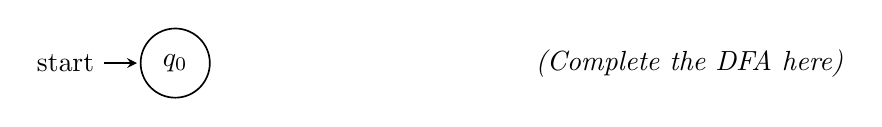
\begin{tikzpicture}[->,>=stealth,shorten >=1pt,auto,node distance=2.8cm,
                      semithick]
    \node[state, initial] (q0) {$q_0$};
    \node[draw=none, right=4cm of q0] {\textit{(Complete the DFA here)}};
  \end{tikzpicture}
  \end{center}

  \vspace{4cm}
  \noindent\textbf{Transition Table:}

  \vspace{0.4cm}
  \begin{center}
  \begin{tabular}{c|c|c}
    \toprule
    \textbf{State} & \textbf{Input 0} & \textbf{Input 1} \\
    \midrule
    $q_0$ (start) & & \\[8pt]
    $q_1$         & & \\[8pt]
    $q_2$         & & \\[8pt]
    $q_3$ (dead)  & & \\[8pt]
    \bottomrule
  \end{tabular}
  \end{center}

  \part[8] Write a \textbf{Regular Expression} for $L$ and briefly explain how it
  corresponds to the DFA you drew.

  \vspace{5cm}
\end{parts}

\newpage

%------------------------------------------------------------
% Problem 2 – FIRST / FOLLOW Sets and LL(1) Parse Table
%------------------------------------------------------------
\question[25]
\textbf{FIRST Sets, FOLLOW Sets, and LL(1) Parse Table}

\medskip
\noindent Consider the following context-free grammar $G$:

\begin{align*}
  S  &\;\longrightarrow\; A\,B\,\$\$ \\
  A  &\;\longrightarrow\; \texttt{a}\,A \;\mid\; \epsilon \\
  B  &\;\longrightarrow\; \texttt{b}\,B\,\texttt{c} \;\mid\; \texttt{d}
\end{align*}

\begin{parts}
  \part[8] Compute $\text{FIRST}(X)$ for each non-terminal $X \in \{S, A, B\}$.
  Show all steps.

  \vspace{6cm}

  \part[8] Compute $\text{FOLLOW}(X)$ for each non-terminal $X \in \{S, A, B\}$.
  Show all steps.

  \vspace{6cm}

  \part[9] Construct the \textbf{LL(1) parse table} for $G$.
  Explain how each table entry was derived using the FIRST and FOLLOW sets
  you computed above.

  \vspace{0.4cm}
  \begin{center}
  \begin{tabular}{c|c|c|c|c|c}
    \toprule
    \multirow{2}{*}{\textbf{Non-terminal}} &
    \multicolumn{5}{c}{\textbf{Current Input Token}} \\
    \cmidrule{2-6}
     & \texttt{a} & \texttt{b} & \texttt{c} & \texttt{d} & \texttt{\$\$} \\
    \midrule
    $S$ & & & & & \\[10pt]
    $A$ & & & & & \\[10pt]
    $B$ & & & & & \\[10pt]
    \bottomrule
  \end{tabular}
  \end{center}

  \vspace{4cm}
\end{parts}

\newpage

%------------------------------------------------------------
% Problem 3 – LR(1) Parsing
%------------------------------------------------------------
\question[25]
\textbf{LR(1) Items, DFA, and Parse Table}

\medskip
\noindent Consider the following \textbf{augmented} context-free grammar $G'$
for a simple expression language with assignment:

\begin{align*}
  (0)\quad S'  &\;\longrightarrow\; S \\
  (1)\quad S   &\;\longrightarrow\; \texttt{id} \;\texttt{:=}\; E \\
  (2)\quad S   &\;\longrightarrow\; E \\
  (3)\quad E   &\;\longrightarrow\; E \;+\; T \\
  (4)\quad E   &\;\longrightarrow\; T \\
  (5)\quad T   &\;\longrightarrow\; T \;\ast\; F \\
  (6)\quad T   &\;\longrightarrow\; F \\
  (7)\quad F   &\;\longrightarrow\; \texttt{(}\; E \;\texttt{)} \\
  (8)\quad F   &\;\longrightarrow\; \texttt{id}
\end{align*}

\noindent The terminal symbols are:
$\{\,\texttt{id},\;\texttt{:=},\;+,\;\ast,\;\texttt{(},\;\texttt{)},\;\$\,\}$.
The non-terminals are $\{S', S, E, T, F\}$.

\begin{parts}
  \part[12] Construct the \textbf{LR(1) canonical collection} of item sets
  $I_0, I_1, \ldots$\,.
  For each item set show all LR(1) items $[A \to \alpha \bullet \beta,\; a]$
  with their lookahead tokens, and indicate all \textsc{goto} transitions.
  \textit{Hint: The automaton has approximately 12--14 states.}

  \vspace{11cm}

  \part[13] Using the item sets from part~(a), construct the complete
  \textbf{LR(1) parse table} (ACTION and GOTO columns).
  Use: $s_n$ = shift to state $n$;\; $r_k$ = reduce by production $(k)$;\;
  \textit{acc} = accept;\; blank = error.

  \vspace{0.3cm}
  \begin{center}
  \renewcommand{\arraystretch}{1.4}
  \begin{tabular}{c|c|c|c|c|c|c|c|c|c|c}
    \toprule
    \multirow{2}{*}{\textbf{State}} &
    \multicolumn{7}{c|}{\textbf{ACTION}} &
    \multicolumn{3}{c}{\textbf{GOTO}} \\
    \cmidrule{2-11}
     & \texttt{id} & \texttt{:=} & $+$ & $\ast$ & \texttt{(} & \texttt{)} & \$ & $S$ & $E$ & $T$ \\
    \midrule
    0  & & & & & & & & & & \\
    1  & & & & & & & & & & \\
    2  & & & & & & & & & & \\
    3  & & & & & & & & & & \\
    4  & & & & & & & & & & \\
    5  & & & & & & & & & & \\
    6  & & & & & & & & & & \\
    7  & & & & & & & & & & \\
    8  & & & & & & & & & & \\
    9  & & & & & & & & & & \\
    10 & & & & & & & & & & \\
    11 & & & & & & & & & & \\
    12 & & & & & & & & & & \\
    \bottomrule
  \end{tabular}
  \end{center}

  \vspace{0.4cm}
  \noindent\textit{Add rows as needed if your automaton has more states.}

  \vspace{1cm}
\end{parts}

\newpage

%------------------------------------------------------------
% Problem 4 – S-Attributed Grammar (Bottom-Up Syntax Tree)
%------------------------------------------------------------
\question[15]
\textbf{S-Attributed Grammar -- Bottom-Up Syntax Tree}

\medskip
\noindent The following is an \textbf{S-attributed} (bottom-up) attribute grammar
for building syntax trees of simple additive expressions:

\begin{align*}
  (1)\quad E_1 &\;\longrightarrow\; E_2 \;+\; T
    &\triangleright\quad& E_1.\mathit{ptr} := \textsc{make\_bin\_op}(\text{``+''}, E_2.\mathit{ptr}, T.\mathit{ptr}) \\[4pt]
  (2)\quad E_1 &\;\longrightarrow\; E_2 \;-\; T
    &\triangleright\quad& E_1.\mathit{ptr} := \textsc{make\_bin\_op}(\text{``$-$''}, E_2.\mathit{ptr}, T.\mathit{ptr}) \\[4pt]
  (3)\quad E   &\;\longrightarrow\; T
    &\triangleright\quad& E.\mathit{ptr} := T.\mathit{ptr} \\[4pt]
  (4)\quad T   &\;\longrightarrow\; (\; E \;)
    &\triangleright\quad& T.\mathit{ptr} := E.\mathit{ptr} \\[4pt]
  (5)\quad T   &\;\longrightarrow\; \textbf{num}
    &\triangleright\quad& T.\mathit{ptr} := \textsc{make\_leaf}(\mathit{num.val})
\end{align*}

\medskip
\noindent Note: $E$ handles addition and subtraction; $T$ is either a
parenthesized expression or a numeric literal.
Multiplication and division are \emph{not} part of this grammar.

\medskip
\noindent Using the grammar above, construct the \textbf{annotated bottom-up parse
tree} and the resulting \textbf{syntax tree} for the expression:
\[
  (5 + 3) - 2
\]

\medskip
\noindent Show each \textbf{reduction step} in order, state which production
(1)--(5) is applied, and write out the \textbf{semantic action} that creates
each syntax tree node. Draw the final syntax tree clearly.

\vspace{12cm}

\newpage

%------------------------------------------------------------
% Problem 5 – L-Attributed Grammar (Top-Down Syntax Tree)
%------------------------------------------------------------
\question[15]
\textbf{L-Attributed Grammar -- Top-Down Syntax Tree}

\medskip
\noindent The following is an \textbf{L-attributed} (top-down) attribute grammar
for building syntax trees.  The attribute $\mathit{st}$ is an
\emph{inherited} attribute passed down the parse tree; $\mathit{ptr}$ is a
\emph{synthesized} attribute passed up.

\begin{align*}
  E   &\;\longrightarrow\; T\;TT
    &\triangleright\quad& TT.\mathit{st} := T.\mathit{ptr};\quad E.\mathit{ptr} := TT.\mathit{ptr} \\[4pt]
  TT_1 &\;\longrightarrow\; +\;T\;TT_2
    &\triangleright\quad& TT_2.\mathit{st} := \textsc{make\_bin\_op}(\text{``+''}, TT_1.\mathit{st}, T.\mathit{ptr});\\
   &&& TT_1.\mathit{ptr} := TT_2.\mathit{ptr} \\[4pt]
  TT_1 &\;\longrightarrow\; -\;T\;TT_2
    &\triangleright\quad& TT_2.\mathit{st} := \textsc{make\_bin\_op}(\text{``$-$''}, TT_1.\mathit{st}, T.\mathit{ptr});\\
   &&& TT_1.\mathit{ptr} := TT_2.\mathit{ptr} \\[4pt]
  TT  &\;\longrightarrow\; \epsilon
    &\triangleright\quad& TT.\mathit{ptr} := TT.\mathit{st} \\[4pt]
  T   &\;\longrightarrow\; F\;FT
    &\triangleright\quad& FT.\mathit{st} := F.\mathit{ptr};\quad T.\mathit{ptr} := FT.\mathit{ptr} \\[4pt]
  FT_1 &\;\longrightarrow\; \ast\;F\;FT_2
    &\triangleright\quad& FT_2.\mathit{st} := \textsc{make\_bin\_op}(\text{``$\times$''}, FT_1.\mathit{st}, F.\mathit{ptr});\\
   &&& FT_1.\mathit{ptr} := FT_2.\mathit{ptr} \\[4pt]
  FT_1 &\;\longrightarrow\; /\;F\;FT_2
    &\triangleright\quad& FT_2.\mathit{st} := \textsc{make\_bin\_op}(\text{``$\div$''}, FT_1.\mathit{st}, F.\mathit{ptr});\\
   &&& FT_1.\mathit{ptr} := FT_2.\mathit{ptr} \\[4pt]
  FT  &\;\longrightarrow\; \epsilon
    &\triangleright\quad& FT.\mathit{ptr} := FT.\mathit{st} \\[4pt]
  F   &\;\longrightarrow\; (\;E\;)
    &\triangleright\quad& F.\mathit{ptr} := E.\mathit{ptr} \\[4pt]
  F   &\;\longrightarrow\; \textbf{const}
    &\triangleright\quad& F.\mathit{ptr} := \textsc{make\_leaf}(\mathit{const.val})
\end{align*}

\medskip
\noindent Using the grammar above, construct the \textbf{annotated top-down parse
tree} and the resulting \textbf{syntax tree} for the expression:
\[
  8 / (2 + 2) \ast 3
\]

\medskip
\noindent Show each \textbf{expansion step}, the inherited and synthesized
attribute values as they are computed, and draw the final syntax tree clearly.

\vspace{10cm}

\newpage

%------------------------------------------------------------
% Reference Page
%------------------------------------------------------------
\question*{\textbf{Reference Page} (No points -- for reference only)}

\noindent\rule{\textwidth}{0.4pt}

\subsection*{Key Definitions}

\noindent\textbf{FIRST Set:} $\text{FIRST}(\alpha)$ is the set of terminals that
begin strings derivable from $\alpha$.  If $\alpha \Rightarrow^* \epsilon$, then
$\epsilon \in \text{FIRST}(\alpha)$.

\medskip
\noindent\textbf{FOLLOW Set:} $\text{FOLLOW}(A)$ is the set of terminals $a$ such
that $S \Rightarrow^* \cdots A\,a\cdots$.  The end-of-input marker \$\$ is always
in $\text{FOLLOW}(S')$.

\medskip
\noindent\textbf{LL(1) Table Construction Rule:}
For each production $A \to \alpha$:
\begin{enumerate}[label=\alph*.]
  \item For each terminal $a \in \text{FIRST}(\alpha)$, add $A \to \alpha$ to
        $M[A,\,a]$.
  \item If $\epsilon \in \text{FIRST}(\alpha)$, then for each terminal
        $b \in \text{FOLLOW}(A)$, add $A \to \alpha$ to $M[A,\,b]$.
\end{enumerate}

\medskip
\noindent\textbf{LR(1) Item:} $[A \to \alpha \bullet \beta,\; a]$ where $a$ is
a lookahead terminal.

\medskip
\noindent\textbf{LR(1) Closure:} If $[A \to \alpha \bullet B\,\beta,\; a]$ is in
the set, add $[B \to \bullet\gamma,\; b]$ for all $B \to \gamma$ and
$b \in \text{FIRST}(\beta\,a)$.

\medskip
\noindent\textbf{LR(1) GOTO:} $\text{GOTO}(I, X) = \text{closure}(\{[A \to \alpha
X \bullet \beta, a] \mid [A \to \alpha \bullet X\,\beta, a] \in I\})$.

\medskip
\noindent\rule{\textwidth}{0.4pt}

\subsection*{Regular Expression Operators}

\begin{tabular}{lll}
  \toprule
  \textbf{Operator} & \textbf{Meaning} & \textbf{Example} \\
  \midrule
  $r^*$   & Zero or more repetitions of $r$  & $0^* = \epsilon, 0, 00, 000, \ldots$ \\
  $r^+$   & One or more repetitions of $r$   & $0^+ = 0, 00, 000, \ldots$ \\
  $r?$    & Zero or one occurrence of $r$    & $0? = \epsilon \text{ or } 0$ \\
  $r_1 \mid r_2$ & Union (alternation)       & $0 \mid 1$ matches $0$ or $1$ \\
  $r_1\,r_2$  & Concatenation              & $01$ matches the string $01$ \\
  $(r)$   & Grouping                         & $(01)^*$ = even-length alternating \\
  \bottomrule
\end{tabular}

\end{questions}

\end{document}
